\subsection{Process analysis}

Analyzing the application proved to be quite difficult, it seemed to have been able to undermine the Android profiler options.  
Android API version 23 without the Google API’s seemed to be the only one able to profile and run the app after trying multiple Android versions. 

The application would steadily run at 88 MB sometimes dipping to 80 MB’s and spiking to 90 MB’s. 
The CPU usage was more prone to spiking and dipping from the low 20\% to spikes of around the 50\% CPU usage. 
The app would generally stay around the 33\% CPU usage.

\begin{figure}[H]
    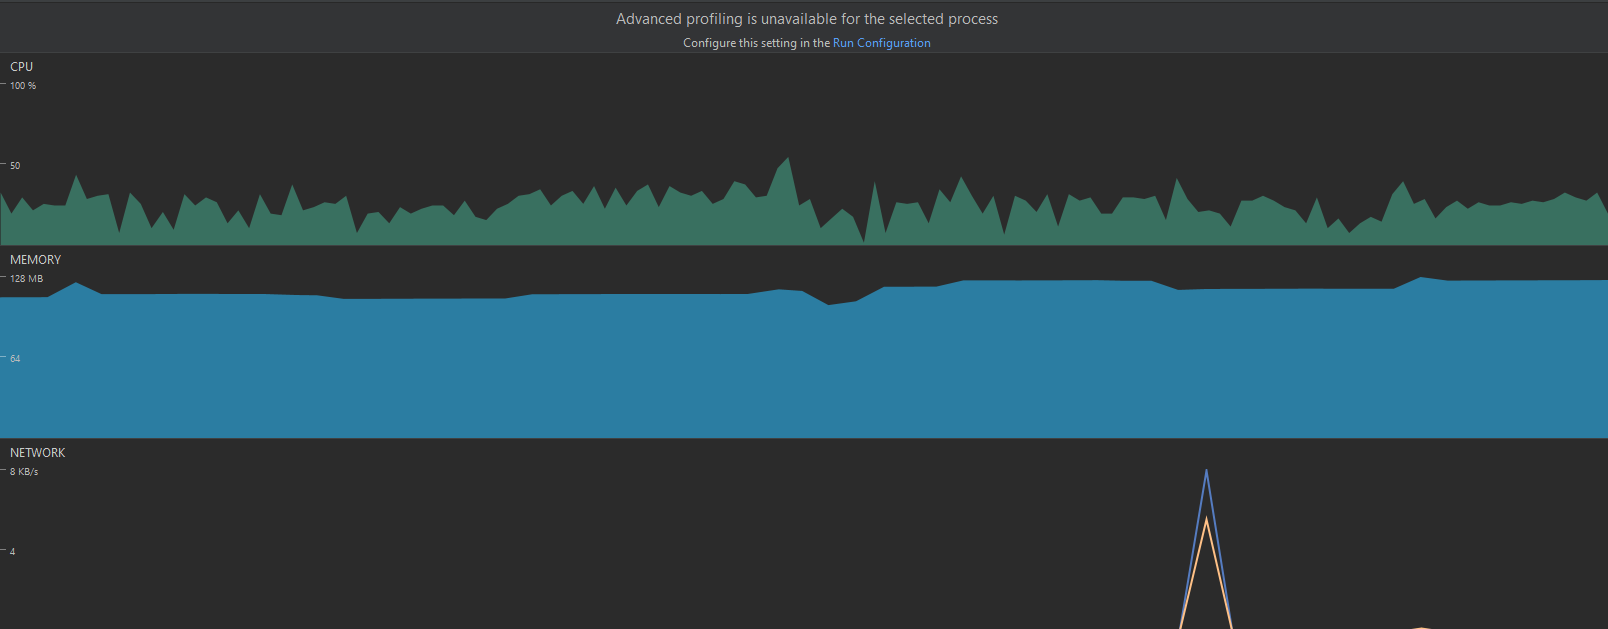
\includegraphics[width=1\textwidth]{processrecording.PNG}
    \caption{Usage of malicious application}
    \label{tim-process}
\end{figure}

As seen on figure \ref{tim-process} it would seem that the application periodically send and received packets via the internet, communicating with the Cloudflare IP. 
The app would however crash after trying to enable the Chrome in the settings menu when it was being profiled. 
This would not occur when the app is run normally without a profiler active. 